\documentclass[tikz]{standalone}
\usetikzlibrary{calc,trees,positioning,arrows,chains,shapes.geometric,%
    decorations.pathreplacing,decorations.pathmorphing,shapes,%
    matrix,shapes.symbols,fit}
\usepackage{ifthen}
\pgfdeclarelayer{back}
\pgfsetlayers{back,main}


\makeatletter
\tikzset{
  fitting node/.style={
    inner sep=0pt,
    fill=none,
    draw=none,
    reset transform,
    fit={(\pgf@pathminx,\pgf@pathminy) (\pgf@pathmaxx,\pgf@pathmaxy)}
  },
  reset transform/.code={\pgftransformreset}
}
\makeatother


\begin{document}
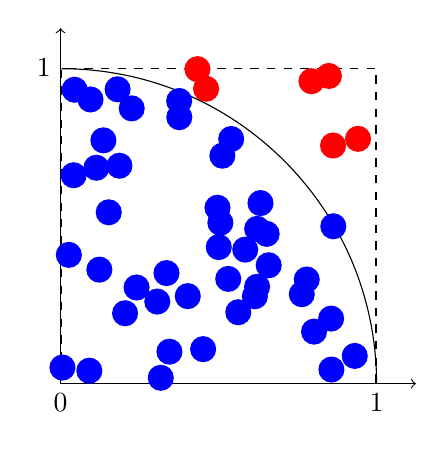
\begin{tikzpicture}

  \node [draw,rectangle,dashed,minimum width=4cm,minimum height=4cm,anchor=south west] at(0.,0.) (unit_box) {};

  \node [left] at(unit_box.north west) (ylabel) {$1$};
  \node [below] at(unit_box.south east) (xlabel) {$1$};

  \node [below] at(unit_box.south west) (orgin) {$0$};

  \draw[->] (unit_box.south west) -- ($(unit_box.north west)+(0,.5)$);
  \draw[->] (unit_box.south west) -- ($(unit_box.south east)+(.5,0.)$);

  
  \draw (unit_box.south east) arc [start angle = 0, end angle = 90, radius=4cm];

  \pgfmathsetseed{2017}

  \foreach \n in {1,...,50}{
    
    \pgfmathsetmacro{\xcoor}{rnd}% x-coordinate
    \pgfmathsetmacro{\ycoor}{rnd}% y-coordinate
    \pgfmathparse{sqrt(\xcoor*\xcoor + \ycoor*\ycoor) < 1.0 ? int(1) : int(0)}

    \ifnum\pgfmathresult=1 
    \node [circle,minimum size=.5mm,fill=blue] at($(4*\xcoor,4*\ycoor)$) (circle_\n) {};
    \else
    \node [circle,minimum size=.5mm,fill=red] at($(4*\xcoor,4*\ycoor)$) (circle_\n) {};
    \fi
    %\node [circle,fill=\pgfmathifthenelse{ \xcoor < 1.}{blue}{red}] at(\xcoor{},\ycoor{}) (circle_\n) {}
  }

\end{tikzpicture}
\end{document}
